% This text is proprietary.
% It's a part of presentation made by myself.
% It may not used commercial.
% The noncommercial use such as private and study is free
% Sep. 2005 
% Author: Sascha Frank 
% University Freiburg 
% www.informatik.uni-freiburg.de/~frank/
%
% additional usepackage{beamerthemeshadow} is used
%  
%  \beamersetuncovermixins{\opaqueness<1>{25}}{\opaqueness<2->{15}}
%  with this the elements which were coming soon were only hinted


%Modified from author's source by KK
\documentclass{beamer}




\usepackage{beamerthemeshadow}
\usepackage{tikz} 
\usetikzlibrary{arrows,decorations.pathmorphing,backgrounds,fit}  
\usetikzlibrary{shapes,snakes}
\begin{document}
\title{A1 Presentation}  
\author{Ben Athiwaratkun and Keegan Kang}
\date{\today} 

\frame{\titlepage} 

\frame{\frametitle{Presentation Objectives}\tableofcontents} 

\section{Introduction}

\frame{\frametitle{Introduction}
\begin{enumerate}
\item [$\bullet$] Most NLP goals focus on making some kind of prediction about a given text.
\pause
\item [$\bullet$] Our proposal is to see if we can make some kind of prediction about the {\it people} who write these texts (social interaction part of the course!).
\end{enumerate}
}

\section{Research Problem}
\frame{\frametitle{Research Problem}

{\it Can we predict the dynamics of any two active users, based on their previous posts?} \\
\pause
\vspace*{1cm}
We use the Slashdog blog conversations from BC3's blog corpus in our investigation.
}


\frame{\frametitle{Research Problem (in detail)}
\begin{enumerate}
\item We would like to know if we can predict the trend of a thread, given the earliest $k$ comments in the article. %The trend here can be the length, a moderation class, the moderation score, or some derived feature based on the text such as aggressiveness, politeness, etc. 
\pause
\item Given the probability distribution for any user $A$ to create posts of quality, we would like to estimate the conditional probability vector of user $A$, given that some event $\mathcal E$ has occurred.
\end{enumerate}

%Here, $\mathcal E$ could be a shift in topic of the thread, or the entry of a new user.
}

\section{Techniques}

\frame{\frametitle{Proposed techniques to tackle the problem}
\begin{enumerate}
\item Look at frequencies! %We analyze the data to prepare for research question 1 by looking at the frequencies of moderation classes. 
\pause
\item Plot the comment length in each thread to see if there are any discernible patterns. %We represent a thread as a collection of all comments sorted chronologically. An alternative could be to represent a single thread as a path from root to leaf. 
\pause
\item Compare distributions and conditional distributions of several metrics. %To address research question 2, we consider the distribution of the comment length for a given user and compare it with the conditional distribution of comment length of the same user conditioned that another user having posted at least once in the thread. 
\end{enumerate}

%Here, $\mathcal E$ could be a shift in topic of the thread, or the entry of a new user.
}

\frame{\frametitle{Example of metrics}
\begin{enumerate}
\item \cite{Otterbacher} %{While these metrics refer to reviews in particular, we will consider metrics 8-17.},
\pause
\item ``Connectedness", as in \cite{Backstrom+al:13a}, by looking at time intervals
\end{enumerate}

%Here, $\mathcal E$ could be a shift in topic of the thread, or the entry of a new user.
}

\section{Preliminary Results and Interesting Stuff}


%Here, $\mathcal E$ could be a shift in topic of the thread, or the entry of a new user.


\begin{frame}[fragile]\frametitle{Classification Breakdown}

A quick breakdown by category...
\pause 

\begin{verbatim}
{'Troll': 14932, 'Funny': 40672, 'None': 464104, 
'Flamebait': 7456,  'Redundant': 4792, 'Offtopic': 11384,
'Informativ': 40188, 'Interestin':  50168, 
'Insightful': 73864}
\end{verbatim}
\end{frame}

\begin{frame}[fragile]\frametitle{Classification Breakdown}

...and by dominating class (when None is removed)
\pause 

\begin{verbatim}
{'Flamebait': 28, 'Funny': 2316, 'Redundant': 8, 
'Troll': 136,  'Offtopic': 68, 'Insightful': 5540, 
'Interestin': 1824, 'Informativ': 1348}
\end{verbatim}
\pause
We could potentially try to classify the comments with class {\tt None} with some the tools Python provides. 

\end{frame}

\frame{\frametitle{Example of Comment Lengths}
\begin{figure}[h!]
\begin{center}
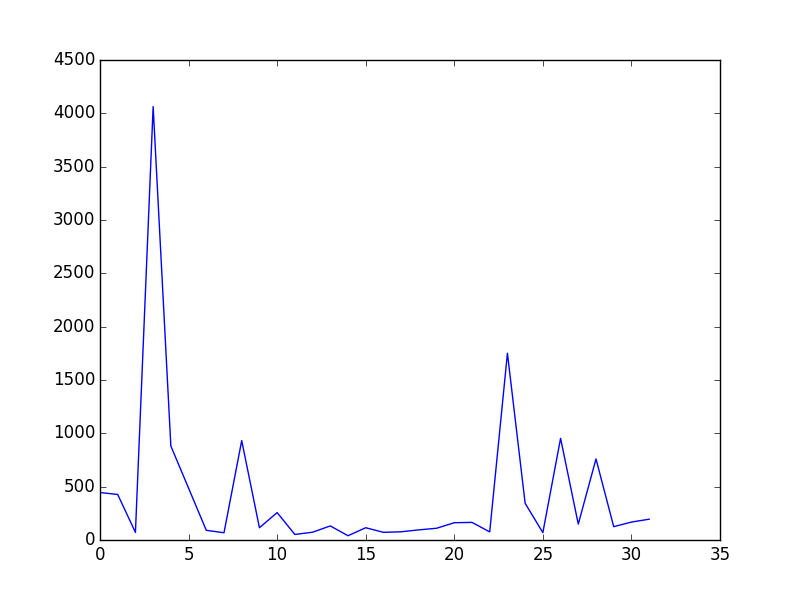
\includegraphics[scale=0.35]{CL_conferencePlagiarism.png}
\caption{Post Length for Article {\tt Conference Board Admits Plagiarism, Pulls Copyright Report}}
\end{center}
\end{figure}
}

\frame{\frametitle{Example of Comment Lengths}
\begin{figure}[h!]
\begin{center}
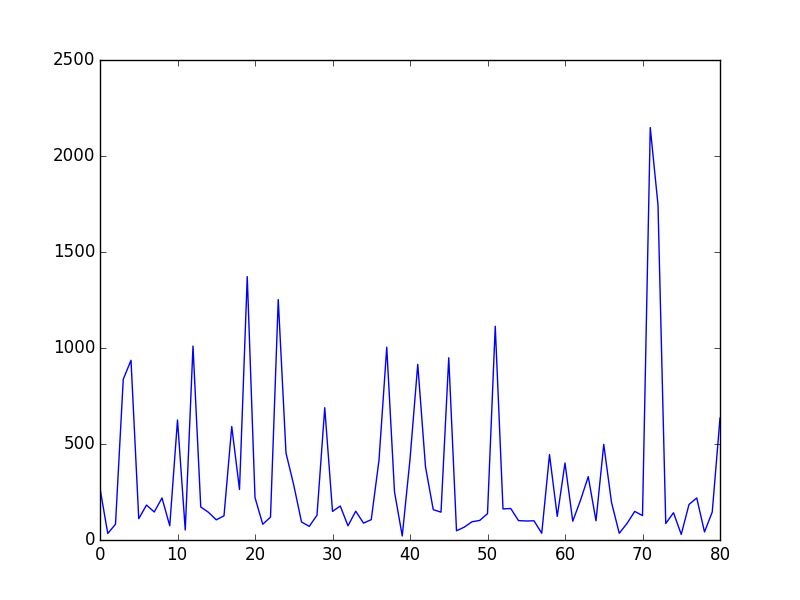
\includegraphics[scale=0.35]{CL_GooglesWave.png}
\caption{Post Length for Article {\tt Google's "Wave" Blurs Chat, Email, Collaboration Software}}
\end{center}
\end{figure}
}

\frame{\frametitle{Distribution and Conditional Distribution of Post Lengths}
\begin{figure}[h!]
\begin{center}
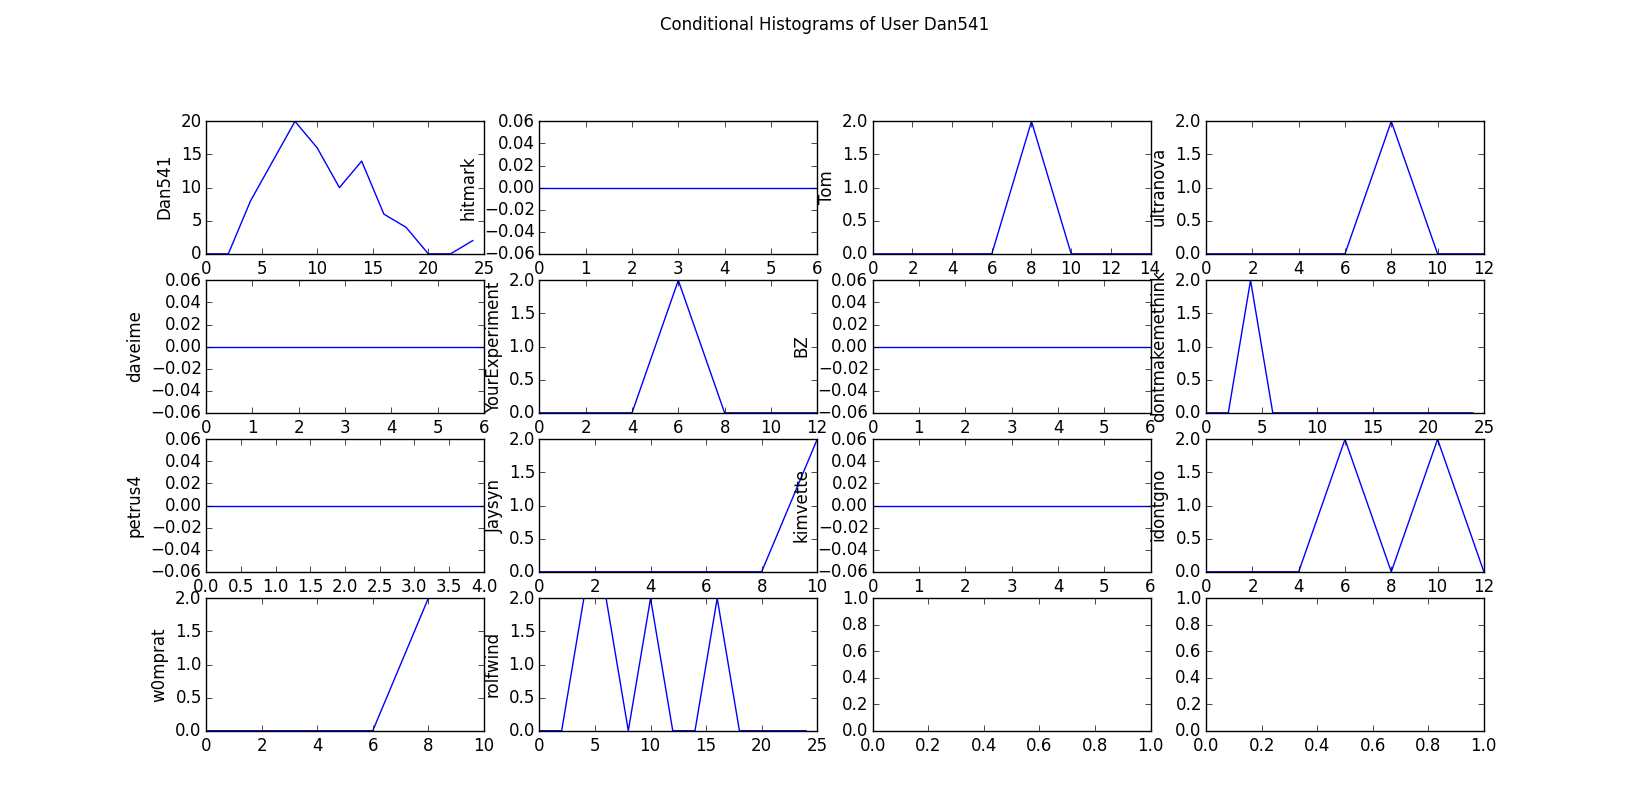
\includegraphics[scale=0.25]{Dan541.png}
\caption{Joint Distribution Plots for user {\tt Dan541} and Other Active User}
\end{center}
\end{figure}
}

\frame{\frametitle{Distribution and Conditional Distribution of Post Lengths}
\begin{figure}[h!]
\begin{center}
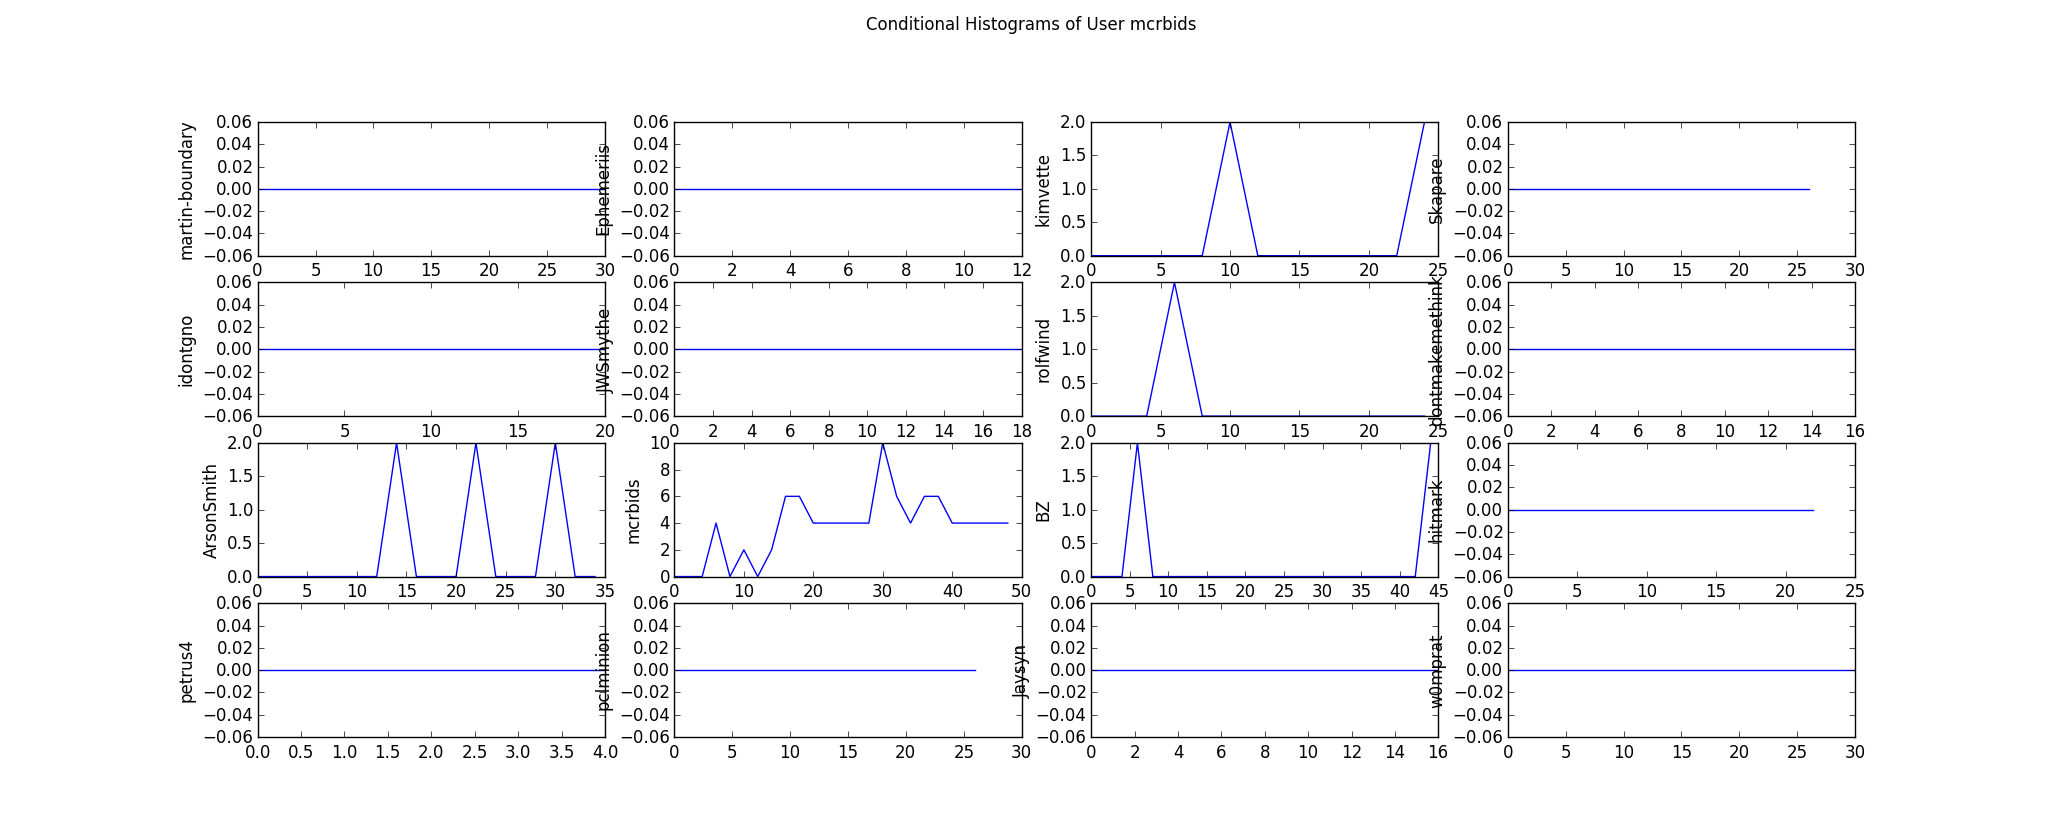
\includegraphics[scale=0.20]{mcrbids.png}
\caption{Joint Distribution Plots for user {\tt mcrbids} and Other Active User}
\end{center}
\end{figure}
}

\frame{\frametitle{Probability and Conditional Probability of Post Type}
\begin{figure}[h!]
\begin{center}
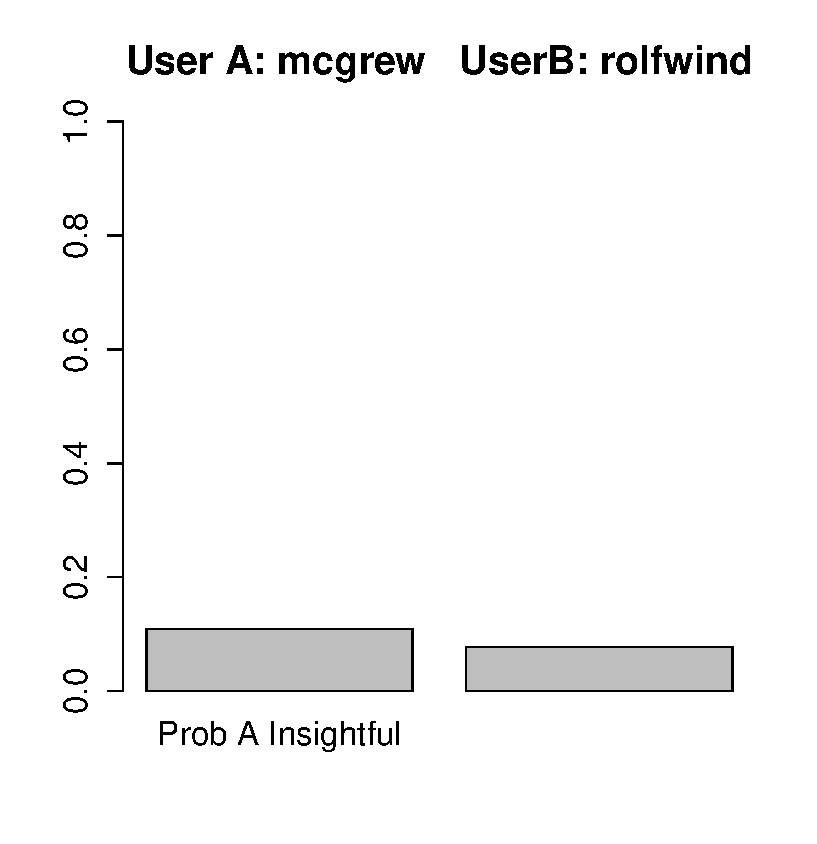
\includegraphics[scale=0.40]{mcgrew-rolfwind.pdf}
\end{center}
\end{figure}
}

\frame{\frametitle{Probability and Conditional Probability of Post Type}
\begin{figure}[h!]
\begin{center}
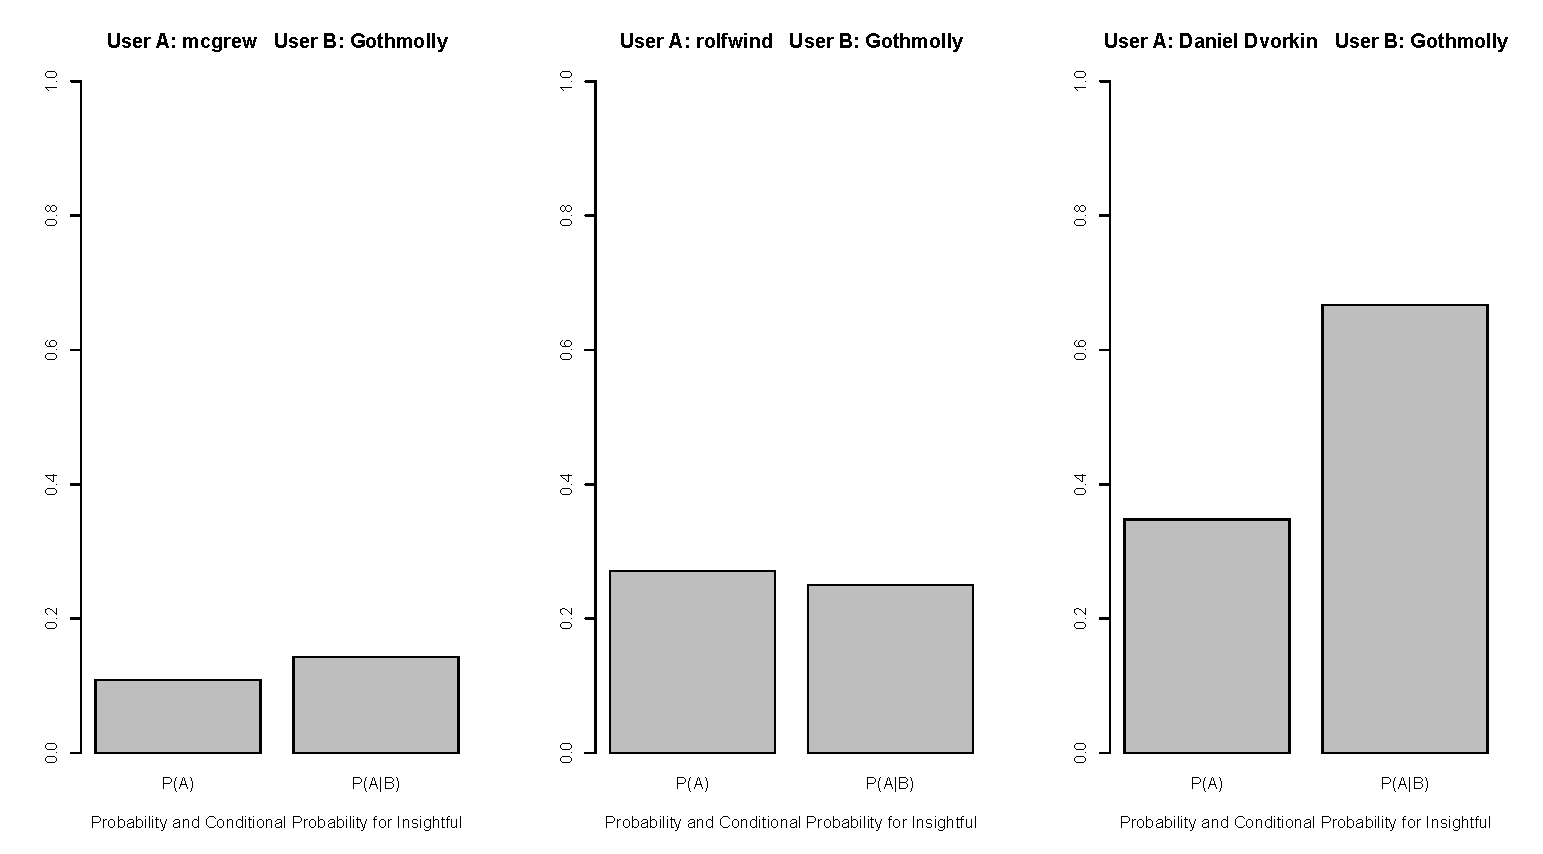
\includegraphics[scale=0.40]{gothmolly.pdf}
\end{center}
\end{figure}
}

\frame{\frametitle{Probability and Conditional Probability of Post Type}
\begin{figure}[h!]
\begin{center}
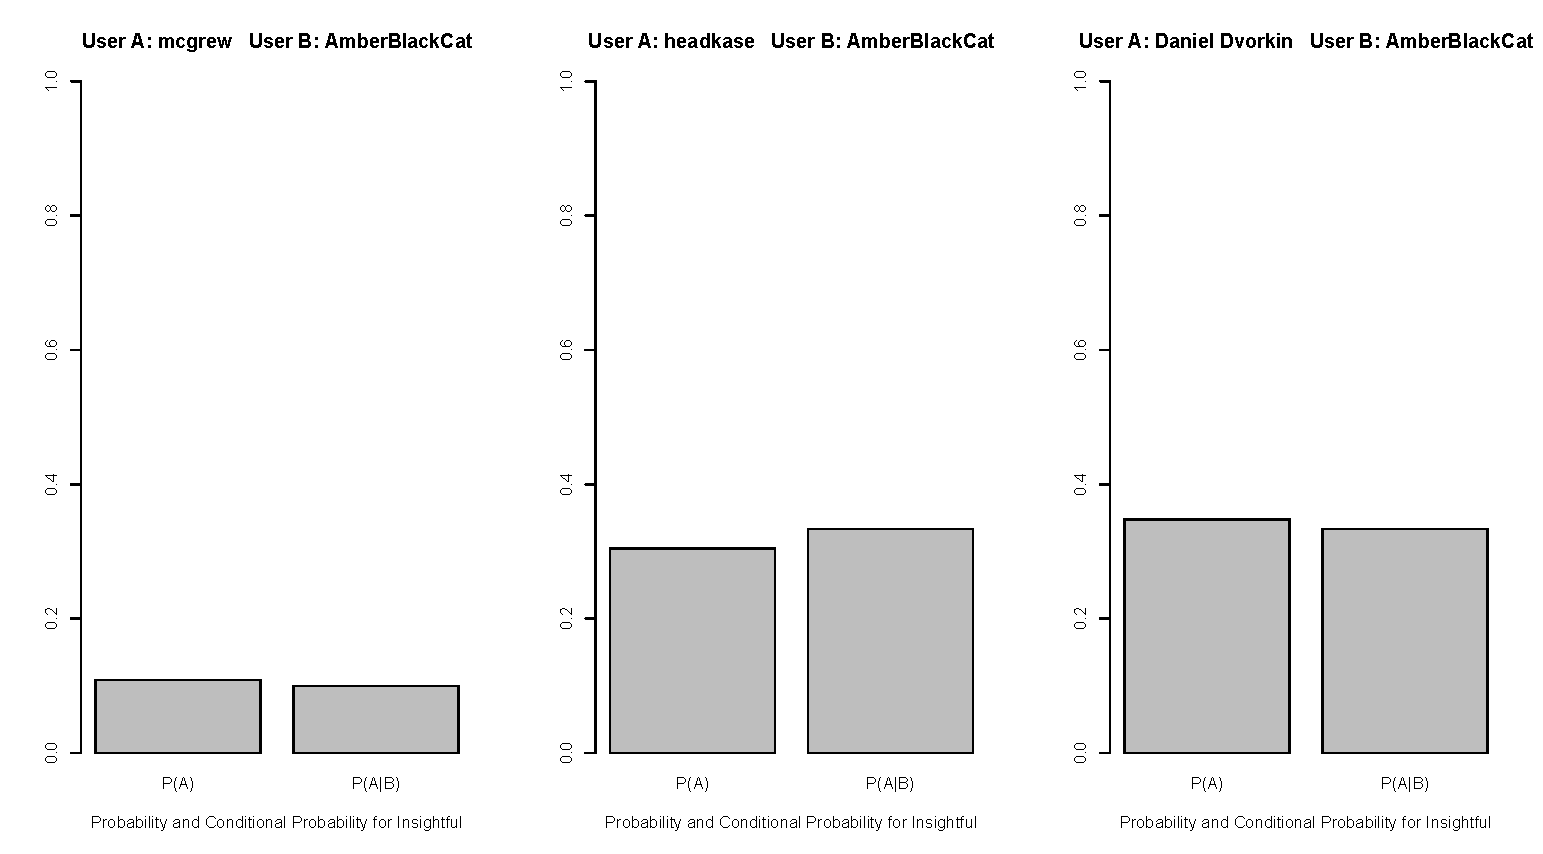
\includegraphics[scale=0.40]{abc.pdf}
\end{center}
\end{figure}
}

\frame{\frametitle{Discussion}
\begin{enumerate}
\item We want to differentiate the real signal from noise.
\pause
\item How can we infer social interaction from a given signal?
\end{enumerate}

}

\bibliographystyle{alpha}	
\bibliography{database}  % expects file "database.bib"

\end{document}



Users: (mcgrew , AmberBlackCat)
The number of posts A made:					864
The number of posts B made:					90
Number of threads B posted:					90
The number of insightful posts A made:				94
Prob A Post Insightful:						0.108796296296
Conditional Probability A Post Insightful with B Present:	0.1


Users: (headkase , AmberBlackCat)
The number of posts A made:					92
The number of posts B made:					90
Number of threads B posted:					90
The number of insightful posts A made:				28
Prob A Post Insightful:						0.304347826087
Conditional Probability A Post Insightful with B Present:	0.333333333333


Users: (Daniel Dvorkin , AmberBlackCat)
The number of posts A made:					92
The number of posts B made:					90
Number of threads B posted:					90
The number of insightful posts A made:				32
Prob A Post Insightful:						0.347826086957
Conditional Probability A Post Insightful with B Present:	0.333333333333



par(mfrow=c(1,3))

tmp =c(0.108796296296, 0.1 )
barplot(tmp, main="User A: mcgrew   User B: AmberBlackCat", ylim=c(0,1), names.arg=c("P(A)","P(A|B)"),xlab ="Probability and Conditional Probability for Insightful")

tmp =c(0.304347826087 ,1/3)
barplot(tmp, main="User A: headkase   User B: AmberBlackCat", ylim=c(0,1), names.arg=c("P(A)","P(A|B)"),xlab ="Probability and Conditional Probability for Insightful")

tmp =c(0.347826086957 ,1/3)
barplot(tmp, main="User A: Daniel Dvorkin   User B: AmberBlackCat", ylim=c(0,1), names.arg=c("P(A)","P(A|B)"),xlab ="Probability and Conditional Probability for Insightful")



Users: (mcgrew , Gothmolly)
The number of posts A made:					864
The number of posts B made:					92
Number of threads B posted:					92
The number of insightful posts A made:				94
Prob A Post Insightful:						0.108796296296
Conditional Probability A Post Insightful with B Present:	0.142857142857



Users: (rolfwind , Gothmolly)
The number of posts A made:					96
The number of posts B made:					92
Number of threads B posted:					92
The number of insightful posts A made:				26
Prob A Post Insightful:						0.270833333333
Conditional Probability A Post Insightful with B Present:	0.25


Users: (Daniel Dvorkin , Gothmolly)
The number of posts A made:					92
The number of posts B made:					92
Number of threads B posted:					92
The number of insightful posts A made:				32
Prob A Post Insightful:						0.347826086957
Conditional Probability A Post Insightful with B Present:	0.666666666667




par(mfrow=c(1,3))

tmp =c(0.108796296296, 0.142857142857 )
barplot(tmp, main="User A: mcgrew   User B: Gothmolly", ylim=c(0,1), names.arg=c("P(A)","P(A|B)"),xlab ="Probability and Conditional Probability for Insightful")

tmp =c(0.270833333333 ,0.25)
barplot(tmp, main="User A: rolfwind   User B: Gothmolly", ylim=c(0,1), names.arg=c("P(A)","P(A|B)"),xlab ="Probability and Conditional Probability for Insightful")

tmp =c(0.347826086957 ,2/3)
barplot(tmp, main="User A: Daniel Dvorkin   User B: Gothmolly", ylim=c(0,1), names.arg=c("P(A)","P(A|B)"),xlab ="Probability and Conditional Probability for Insightful")













Users: (mcgrew , rolfwind)
The number of posts A made:					864
The number of posts B made:					96
Number of threads B posted:					94
The number of insightful posts A made:				94
Prob A Post Insightful:						0.108796296296
Conditional Probability A Post Insightful with B Present:	0.0769230769231

Users: (rolfwind , mcgrew)
The number of posts A made:					96
The number of posts B made:					864
Number of threads B posted:					556
The number of insightful posts A made:				26
Prob A Post Insightful:						0.270833333333
Conditional Probability A Post Insightful with B Present:	0.142857142857

par(mfrow=c(1,2))

tmp =c(0.108796296296,0.0769230769231)
barplot(tmp, main="User A: mcgrew   User B: rolfwind", ylim=c(0,1), names.arg=c("P(A)","P(A|B)"),xlab ="Probability and Conditional Probability for Insightful")

tmp =c(0.270833333333,0.142857142857)
barplot(tmp, main="User A: rolfwind   User B: mcgrew", ylim=c(0,1), names.arg=c("P(A)","P(A|B)"),xlab ="Probability and Conditional Probability for Insightful")







